% hunspell: tex
\documentclass[a4paper,10pt,abstract=true,headings=small]{scrartcl}
\usepackage[lmargin=4cm,rmargin=4cm,tmargin=3cm,bmargin=5.0cm,footskip=1.5cm]{geometry}
\linespread{1.1}

\usepackage[luatexrenderer=Node]{polyglossia}
\setmainlanguage{german}
\setotherlanguage{english}


\usepackage{fontspec}
\usepackage{unicode-math}
%\setmainfont[Scale=1.05]{Libertinus Serif}
\setmainfont[BoldFont=texgyretermes-bold.otf,ItalicFont=texgyretermes-italic.otf]{texgyretermes-regular.otf}
\setmathfont{texgyretermes-math.otf}
\addtokomafont{disposition}{\rmfamily}


\usepackage[hidelinks,pdfusetitle,pdfencoding=auto,psdextra,bookmarksopen]{hyperref}

\usepackage{graphicx}% for \rotatebox
\usepackage{everypage}
\usepackage{environ}
\usepackage{pdflscape}% not required
\usepackage{pdfpages}

\newcounter{abspage}% \thepage not reliab

\makeatletter
\newcommand{\newSFPage}[1]% #1 = \theabspage
  {\global\expandafter\let\csname SFPage@#1\endcsname\null}

\NewEnviron{SidewaysFigure}{\begin{figure*}[p]
\protected@write\@auxout{\let\theabspage=\relax}% delays expansion until shipout
  {\string\newSFPage{\theabspage}}%
\ifdim\textwidth=\textheight
  \rotatebox{90}{\parbox[c][\textwidth][c]{\linewidth}{\BODY}}%
\else
  \rotatebox{90}{\parbox[c][\textwidth][c]{20cm}{\BODY}}%
\fi
\end{figure*}}

\AddEverypageHook{% check if sideways figure on this page
  \ifdim\textwidth=\textheight
    \stepcounter{abspage}% already in landscape
  \else
    \@ifundefined{SFPage@\theabspage}{}{\global\pdfpageattr{/Rotate 0}}%
    \stepcounter{abspage}%
    \@ifundefined{SFPage@\theabspage}{}{\global\pdfpageattr{/Rotate 90}}%
  \fi}
\makeatother



\usepackage[notes,dashed=false]{biblatex-chicago}
\setcounter{biburllcpenalty}{7000}
\setcounter{biburlucpenalty}{8000}
\setlength{\bibitemsep}{0pt}
\addbibresource{references.bib}
\DefineBibliographyStrings{german}{
  andothers        = {et\,al\adddot},
  andmore          = {et\,al\adddot}
}

\usepackage[german=guillemets,autostyle=true]{csquotes}
\SetCiteCommand{\autocite}
\usepackage[format=plain]{caption}
\usepackage[inline]{enumitem}
\setlist{itemsep=0pt,parsep=4pt}
\setlist[enumerate]{label=(\roman*), itemsep=0pt}
\usepackage{mathtools}

\setlength{\emergencystretch}{2em}
\setlength{\parskip}{0pt}
\setlength{\parindent}{.4cm}
\widowpenalty=10000
\clubpenalty=10000

\newcommand{\eng}[1]{\textenglish{\emph{#1}}}
\renewcommand{\dag}{{\scshape dag}}

\author{Anton Ehrmanntraut}
\date{3. März 2021}
\title{Maschinelle Identifikation von Handlungssequenzen in digitalen Editionen dramatischer Texte}
\subtitle{\vspace*{.5cm}Eine netzwerktheoretische Heuristik\vspace*{.5cm}}

\begin{document}
\flushbottom
\maketitle

\begin{abstract}
    Aktuelles Forschungsdesiderat in den literarischen Netzwerkanalyse ist eine effektive Modellierung von Plot bzw. Handlungsabläufen.
    Im Kontext von Dramen werden dabei üblicherweise Figurennetzwerke herangezogen.
    Diese werden in aktuellen Forschungsansätzen durch eine zeitliche Dimension zu dynamischen Figurennetzwerken erweitert, um so Plot-Entwicklungen abzubilden.
    Die hier vorliegende Arbeit wählt einen alternativen Weg und präsentiert statische gerichtete Netzwerke, in der die Szenen bzw. Situationen die Entitäten des Netzwerks bilden, nicht Figuren.
    Gerichtete Kanten im Netzwerk verbinden frühere zu späteren Situationen, wenn eine Figur in den beiden Situationen sukzessiv auftritt.
    Die Arbeit versucht zu verdeutlichen, dass in solchen Netzwerken Handlungssequenzen erkennbar werden.
    Hieraus ergibt sich auf natürliche Weise eine Operationalisierung mittels gewichtsmaximalen disjunkten Wegüberdeckungen, welche aus der Struktur eines Dramas eine Plot-Segmentierung errechnen kann.
    Diese wird anhand \emph{Götz von Berlichingen} vorgeführt und evaluiert.
\end{abstract}


\section{Einleitung}

Franco Moretti kann mit seinem Pamphlet \citetitle{moretti_network_2011}\autocite{moretti_network_2011} als Begründer eines Programms verstanden werden, welches die Quantifikation von Plot innerhalb narrativer Texte mittels Methoden aus den \eng{Digital Literary Studies} zum Ziel hat.
(\emph{Plot} soll hier und im Folgenden nur intuitiv verstanden werden.)
Während Fragen zu \textquote{\eng{language and style}} durch Korpusanalysen in den \emph{Digital Literary Studies} quantitativ und maschinell beantwortet werden können, befindet sich im Rahmen von \textquote{\eng{plot}} immer noch eine Leerstelle. % hunspell: acc language and style plot
% hunspell: add Morettis distant reading 
Ferner ist in Morettis Vorhaben auch eine Motivation in Richtung \eng{distant reading} zu finden: Gerade die computerisierte Methode, Plot auszuwerten, könnte in großen Korpusanalysen generelle Grammatiken bzw. Regularitäten im Plot vieler Werke zum Vorschein bringen. % hunspell: acc -Motivation
Zur Schließung dieser Leerstelle schlägt Moretti vor, die \emph{Netzwerkanalyse} als Instrument zur quantitativen Plot-Analyse heranzuziehen.\autocites[Vgl.][]{moretti_network_2011}[Vgl.][]{trilcke_small_2020}

Im Rahmen Morettis Pamphlets wurde beispielsweise das \emph{Figurennetzwerk} vom dramatischen Werk \emph{Hamlet} betrachtet.
In den Figurennetzwerken bildet das Personal von \emph{Hamlet} die Entitäten, und je zwei Figuren relieren binär (bildlich: sind verbunden), wenn diese auf der Bühne interagieren.\autocite[Siehe z.\,B.][13, Abbildung 1]{moretti_network_2011}
Nach Moretti bilden diese Interaktionen die Handlungen des Dramas ab – das resultierende Figurennetzwerk damit die summative strukturalisierte Gesamthandlung des Werks.
Trilcke greift diese Idee auf, und führt diese mit Mitteln der \emph{Social Network Analysis} rigoros weiter.\autocite{trilcke_social_2013} % hunsepll: acc Social Network Analysis
Es ist klar, dass eine solche reduktionistische Quantifikation nie den reichhaltigen Plot-Begriff vollständig abbilden kann.
Vielmehr soll durch dieses Vorhaben analysiert werden, welche Plot-Aspekte überhaupt aus struktureller Perspektive erklärt werden können.\autocite[Vgl.][176]{trilcke_netzwerkdynamik_2017}

Auch wenn o.\,g. Ergebnisse in die Richtung einer Operationalisierung von Plot gehen, macht Trilcke selbst später darauf aufmerksam, dass die Erfassung von Plot durch diese Figurennetzwerke nicht zufriedenstellend ist.
Nach Trilcke et~al. sei zentrale Schwachstelle, dass Figurennetzwerke als \emph{statische} Modelle die zeitliche Dimension von Plot nicht abbilden können.\autocite[Vgl.][176]{trilcke_netzwerkdynamik_2017}
Die hier vorliegene Arbeit folgt daher ihrem generellem Forschungsdesiderat: Die Netzwerkanalyse im Rahmen von Dramen sei in Richtung einer quantitativen Plot-Analyse weiterzuentwickeln.
Aktuelle Entwicklungen in der Netzwerkanalyse versuchen daher, \emph{dynamische} Netzwerke zu entwickeln, um sie für die Plot-Analyse zu gebrauchen.\autocite[Vgl.][176]{trilcke_netzwerkdynamik_2017}
Diese Arbeit wählt einen alternativen Weg und motiviert Netzwerke für dramatische Texte, in denen die \emph{Auftritte} die Entitäten des Netzwerks darstellen, nicht die Figuren.
Wie in der literarischen Netzwerkanalyse üblich, verwertet die hier vorgestellte Methode ausschließlich strukturelle Aspekte der dramatischen Werke.
Das Modell ist daher blind gegenüber dem Inhalt des Haupttext.

Präziser will die Arbeit Folgendes plausibilisieren: 
\begin{enumerate*}
    \item In solchen Netzwerken werden Handlungssequenzen deutlich.
    \item So lässt sich heuristisch ein Vorschlag zu einer Plot-Strukturierung eines dramatischen Werks errechnen.
\end{enumerate*}
Der letzte Punkt soll insbesondere beitragen, aus dieser Plot-Strukturierung dann Kompositionsprinzipien von Plot in digitalen Korpora messbar zu machen.
Via \eng{distant reading} können dann viele Werke hinsichtlich Plot-Struktur verglichen werden.
So kann bspw. Fragen zum Verhältnis von Haupt- und Nebenhandlung, oder zu Verknüpfungstechniken von Handlungssequenzen für ein großes Korpus nachgegangen werden. % hunspell: acc distant reading


Der nächste Abschnitt konkretisiert Begriffe, die wir zur Erarbeitung des Netzwerkmodells benötigen.
Insbesondere wählen wir einen Handlungs(sequenz)begriff, definieren Begriffe aus der Graphentheorie, und gehen kurz auf das digitale Dramenkorpus \emph{GerDraCor} ein. % hunspell: acc Handlungs sequenz
Anschließend wird in Abschnitt \ref{sec:verwandte-arbeiten} auf verwandte Arbeiten der netzwerktheoretischen Plot-Analyse eingegangen.
Abschnitte \ref{sec:situationsgraph} und \ref{sec:segmentierung} wenden sich dem eigentlichen Ziel zu, und behandeln o.\,g. Punkte (i) und (ii): Erster plausibilisiert das Modell der \emph{Situationsgraphen}, Zweiter erklärt wie sich hieraus eine Plot-Struktur heuristisch errechnen lassen kann.




\section{Grundlagen}\label{sec:grundlagen}

\subsection{Zum Begriff der Handlung in dramatischen Texten}\label{sec:handlung}

Grundsätzlich ist zu sagen, dass der Begriff des Plots bzw. \enquote*{Handlung} nur schwer und aufwändig zu präzisieren ist.\autocites[Vgl.][]{kukkonen_plot_2014}[Vgl.][]{herman_routledge_2005}
Wir wollen deshalb für diese Arbeit deshalb folgende bewusst sehr vereinfachende Arbeitsdefinitionen verwenden: \emph{Gesamthandlung} soll hier für die summative \textquote*{Handlung}  verstanden werden.
Also all den im Text dargestellten Begebenheiten, gewissermaßen als Übersetzung von \emph{mythos} bzw. Fabel.

% hunspell: add Hübler
\emph{Handlung} soll als genau jene \textquote*{Einzelhandlung} bzw. \textquote{Begebenheit} verstanden werden, welche die Gesamthandlung konstituieren.\autocite[Vgl.][5--8]{asmuth_einfuhrung_2016}
Damit sind nicht nur Handlungen im engeren Sinne gemeint (nach Pfister und Hübler eine \textquote{absichtsvoll gewählte, nicht kausal bestimmte Überführung einer Situation in eine andere}\footnote{\cite[269]{pfister_drama:_2001}. \textquote{Situation} im Kontext dieses Zitats entspricht nicht der Verwendung in dieser Arbeit.}). Gemeint sind auch solche \textquote{Begebenheiten}, die überhaupt nicht mehr als Handlungen erkennbar sind, weil an ihnen keine Tätigkeiten von Figuren beteiligt sind, z.\,B. Naturgewalt.
Diese Art von Handlungen würde Pfister eher als \textquote{Geschehen} beschreiben\autocite[Vgl.][270]{pfister_drama:_2001}.
Auf diese feine Aufschlüsselung soll in dieser Arbeit aber verzichtet werden.

Eine \emph{Handlungssequenz} soll für uns mehr als nur eine Aneinanderreihung von Handlungen bezeichnen.
Intuitiv können wir erwarten, dass sinnvolle Handlungssequenzen zusammenhängende Teile der Gesamthandlung umfassen – wobei an dieser Stelle ganz explizit ausgelassen wird, was \textquote{zusammenhängend} bedeuten soll.
Auch wenn aufgrund unseres Handlungsbegriff eine Handlungssequenz mehr erfasst als Pfisters gleichnamiger Sequenzbegriff, bestätigt er diese Intuition: % hunspell: acc Pfisters
\blockcquote[Vgl.][285]{pfister_drama:_2001}{
    % hunspell: off
    Die Gesamtheit der Handlungs- und Geschehenszusammenhänge \textins{\emph{Handlung} in unserem Fall} in 
    einem dramatischen Text läßt sich nicht immer, dem aristotelischen Postulat der \textquote*{Einheit des Mythos} entsprechend (\emph{Poetik}, Kap. 8), auf eine einzige Handlungs- oder Geschehenssequenz \textins{wird in unserem Fall zu \emph{Handlungssequenz} zusammengefasst} zurückführen, sondern beruht meist auf einer Kombination mehrerer \textelp{Handlungssequenzen}. Eine solche Sequenz ist ein in sich relativ geschlossenes System 
chronologischer und kausaler Relationen.
}
% hunspell: on
Den letzten Satz können wir als eine Definition für Handlungssequenzen (in Abgrenzung an willkürliche Sequenzen von Handlungen) auffassen.
Dass Pfister nicht näher darauf eingeht, was er mit \textquote{chronologischen und kausalen Relationen} meint, ist durchaus nicht problematisch.
Wir sehen das als Möglichkeit, \textquote{kausale Relationen} möglichst offen zu verstehen.

\label{page:plot-segmentierung}
Im obigen Zitat wird auch das Ziel der Arbeit deutlich, wie in der Einleitung intuitiv angesprochen:
Die Gesamthandlung eines Dramas ist oft mehr als eine einzige lineare Kette an Einzelhandlungen.
Die Komposition der Handlungssequenzen ist meist durchaus komplexer.
Essenziell für eine Analyse ist daher, diejenigen Handlungssequenzen zu identifizieren, welche kombiniert die Gesamthandlung konstituieren.
Gerade im Hinblick auf Fragen betreffend der hierarchischen Abstufung (\textquote*{Haupthandlung} vs. \textquote*{Nebenhandlung}) ist es vorteilhaft, wenn eine solche Segmentierung thematisch ähnliche Handlungen in Sequenzen zusammenfasst.
Bzw. wenn die resultierenden Sequenzen der Segmentierung sich thematisch und kausal abgrenzen.
Eine sinnvolle Segmentierung ist deshalb auch möglichst grob, also bestehend aus aus langen, stark zusammenhängenden, wenigen Handlungssequenzen.

\subsection{Segmentierung der Darstellung in Situationen}\label{sec:situationen}

Auf der Seite der Darstellung definieren wir eine \emph{Situation} – hier nun Marcus folgend – als Segmentierung des Textverlaufs in Abschnitte, in denen keine Veränderungen hinsichtlich der Szenerie oder den präsenten Figuren erfolgen.
Situationen werden also durch Szenenwechsel sowie das Auf- oder Abtreten einer Figur begrenzt.\autocite[Vgl.][140]{marcus_mathematisch-linguistisches_1971} % hunspell: acc Auf-

Durch unsere Definition sprechen wir Handlungen einen punktuellen Charakter zu.
Im Folgenden werden wir daher annehmen, dass wir jeder Situation einer Menge von Handlungen zuordnen können.
Insbesondere erstreckt sich eine Handlung nicht über mehrere Situationen. 
Es sei hier außerdem angemerkt, dass die Umkehrung obiger Annahme nicht zutrifft: Eine Handlung des Dramas muss im Allgemeinen nicht immer in einer Situation dargestellt werden.
Eine Handlung kann auch \emph{verdeckt} an der Gesamthandlung beteiligt sein.
Darunter fallen neben den \emph{räumlich} verdeckten Handlungen (z.\,B. Mauerschau) auch die \emph{zeitlich} verdeckten Handlungen (welche z.\,B. ausgespart wurden und nicht szenisch präsentiert werden).
Üblicherweise werden solche Handlungen dann narrativ von den Figuren vermittelt.\autocite[Vgl.][276]{pfister_drama:_2001}

\subsection{Personal und Rede}\label{sec:personal}

Nachdem der Begriff der Handlung für unser Vorhaben geklärt wurde, führen wir im Kontext dramatischer Texte abschließend noch einige Begriffe zum Personal und zur Handlung ein.
Entsprechend unserer Definition definiert eine \emph{Situation} eindeutig eine Teilmenge von Figuren, welche zur entsprechenden Situation auf der Bühne präsent sind.
Diese Teilmenge nennen wir die zur spezifischen Situation korrespondierende \emph{Konfiguration}.\autocite[Vgl.][235]{pfister_drama:_2001}
% hunspell: add Repliken Replik Replikenlänge
Zu einer spezifischen Situation und einer spezifischen Figur sei die \emph{Replikenlänge} die Anzahl Wörter aller Redebeiträge dieser Figur in der vorgegebenen Situation.
Wenn diese Figur nicht in der korrespondierenden Situation auftreten sollte, ist die Replikenlänge Null.


\subsection{Zur Datengrundlage}\label{sec:daten}

Grundlage der literarischen Netzwerkanalyse ist die Abstraktion der \emph{Struktur} dramatischer Texte.
Der Inhalt des Haupttextes wird dabei ignoriert bzw. nur rudimentär quantitativ ausgewertet.
Das liegt schon daran, dass Fragestellungen betreffend des Inhalts nicht bzw. nur rudimentär maschinell beantwortet werden können, und sich deshalb den \eng{Digital Literary Studies} weitestgehend entzieht.\autocite[Vgl.~auch][607]{jannidis_computergestuetzte_2017}

Stattdessen wird auf auf manuell annotierte digitale Editionen dramatischer Texte zurückgegriffen.
Diese zeichnen zu einem Dramentext die Sprechakte aus, und unterteilen das Werk in strukturelle Einheiten anhand der Überschriften bzw. des Nebentextes.
In unserem Fall verwenden wir hierfür das \emph{German Drama Corpus (GerDraCor)}\footnote{\cite{fischer_programmable_2019}.\par Wenn im Folgenden auf \emph{GerDraCor}-Editionen Bezug genommen wird, dann ist immer die Revision e0da4e0 (20.~Februar 2021) des Git-Repositories gemeint: \url{https://github.com/dracor-org/gerdracor/tree/e0da4e0a181b577326cc8c69adf86e8cd8e94433}}, eine Sammlung TEI-codierter deutscher dramatische Werke. % hunspell: acc Git-Repositories Corpus German -Editionen
Aus der entsprechenden XML-Datei lässt sich so die im Nebentext ausgezeichnete Akt- und Szenenabfolge des Werks bestimmen, sowie die einzelnen Repliken jeder Figur.
Hieraus wollen wir die oben definierte Struktur eines dramatischen Werks wie folgt ableiten:
\begin{enumerate*}
    \item Jede Szene entspricht genau einer Situation.
        Wir gehen also davon aus, dass während der Szene keine Veränderung der präsenten Figuren erfolgt.
    \item Die Konfiguration einer Situation/Szene ergibt sich aus den Replikenmenge der Szene. % hunspell: acc Replikenmenge
        Wir nehmen also an, dass nur jene Figuren auf der Bühne in einer Szene präsent sind, welche auch sprechen.
\end{enumerate*}

Es ist klar, dass diese Annahmen im Allgemeinen nicht zutreffen.
Dieser Reduktionismus sei aber im Hinblick auf eine quantitative Auswertung großer digitaler TEI-genormter Korpora wie \emph{GerDraCor} ausgewählt.
Eine potentielle Operationalisierung muss mit diesen Imperfektionen der Eingangsdaten umgehen.


\subsection{Graphen}

Wir folgen den Ausführungen von Krumke und Noltemeier für eine formal präzise Definition des Graphen.
Ein \emph{gerichteter Graph} (kurz \emph{Graph}) ist ein Quadrupel $G=(V,R,\alpha, \omega)$ mit folgenden zwei Eigenschaften:
\begin{enumerate*}
    \item Die Mengen $V$ und $R$ sind endlich und disjunkt.
        Erstere wird als \emph{Eckenmenge} bezeichnet, letztere als \emph{Pfeilmenge}.
    \item Die Funktionen $\alpha$ und $\omega$ bilden von $R$ nach $V$ ab.
        Für $r\in R$ sagen wir, dass $r$ \emph{von $\alpha(r)$ nach $\omega(r)$ zeigt}.
\end{enumerate*}


Ein Pfeil $r$ nennen wir \emph{Schlinge} wenn $\alpha(r)=\omega(r)$. Zwei Pfeile $r, r'$ nennen wir \emph{parallel}, wenn $\alpha(r)=\alpha(r')$, $\omega(r)=\omega(r')$.
Ein Graph ist \emph{einfach}, wenn seine Pfeilmenge weder Schlingen noch Parallelen enthält.\autocite[Vgl.][7--8]{krumke_graphentheoretische_2012}
Zur einfacheren Notation bezeichnen wir für gegebenen Graph $G$ mit $V(G)$ bzw. $R(G)$ die zu $G$ zugehörige Ecken- bzw. Pfeilmenge. % hunspell: acc Ecken-

Ein \emph{Weg} $P$ ist eine endliche Folge $(v_0,\allowbreak r_1,\allowbreak v_1, \dots, r_k, v_k)$, $k\geq 0$, sodass $v_0, \dots, v_k$ Ecken sind, $r_1, \dots, r_k$ Pfeile sind, sowie $\alpha(r_i) = v_{i-1}$, $\omega(r_i)=v_i$ für alle $i=1,\dots, k$.
Wir sagen, dass $P$ die Ecken $v_0, \dots, v_k$ bzw. Pfeile $r_1, \dots, r_k$ \emph{durchläuft}.
Mit $R(P)$ bezeichnen wir die Menge an durchlaufenen Pfeilen.
Die \emph{Länge} des Wegs $P$ ist $k$, also die Anzahl der durchlaufenen Pfeile.
Man beachte, dass auch $(v_0)$ ein Weg (der Länge $0$) ist.\autocite[Vgl.][31]{krumke_graphentheoretische_2012}

Ein \emph{gerichteter azyklischer Graph} ist ein Graph, welcher keinen Kreis enthält.
Also in dem kein Weg $P=(v_0, \dots, v_k)$ mit $k\geq 1$ existiert, sodass $v_0=v_k$.
In dieser Klasse von Graphen definieren wir – dem Terminus von Diestel folgend – eine \emph{(ecken-\nolinebreak{})disjunkte Wegüberdeckung} für einen gerichteten azyklischen Graph $G$ als eine Menge von Wegen $\mathcal{P}$, sodass jede Ecke $v\in V(G)$ von genau einem Weg $P\in\mathcal{P}$ durchlaufen wird.\autocite[55]{diestel_graphentheorie_2006} % hunspell: acc ecken-


\section{Verwandte Arbeiten}\label{sec:verwandte-arbeiten}

\subsection{Analyse der Konfigurationsstruktur}

Pfister und Asmuth etablieren die Analyse der Konfigurationsstruktur eines Dramas mittels Marcus' \emph{Konfigurationsmatrizen} als Werkzeug \textquote*{traditioneller} Literaturwissenschaft, insbesondere im Hinblick auf Figuren- und Handlungsanalysen. % hunspell: acc Figuren-
Jede Zeile dieser Matrix repräsentiert hierbei eine Figur, jede Spalte eine Situation und die korrespondierende Konfiguration.
Wenn immer also eine Figur in einer spezifischen Situation auftritt, steht in der korrespondierenden Zelle eine 1, ansonsten 0.\autocites[Vgl.][140--141]{marcus_mathematisch-linguistisches_1971}[Vgl.][236--240]{pfister_drama:_2001}[Vgl.][44--47]{asmuth_einfuhrung_2016}

Auch die Betrachtung von Figurennetzwerken kann als Teil dieser Konfigurationsanalyse betrachtet werden.\footnote{Das ist schon deshalb naheliegend, als da Konfigurationsmatrix $M$ und Adjazenzmatrix des Figurennetzwerk $A$ offenbar in der Beziehung $MM^\intercal=A$ stehen. \cite[Siehe auch][201--203, 221--222]{trilcke_social_2013}. Vgl. auch $M(\Omega)$, $G(\Omega)$ bei \cite[140--142]{marcus_mathematisch-linguistisches_1971}.}
Entscheidend ist, dass die Perspektivierung aus der Netzwerkanalyse/-visualisierung (Moretti) bzw. \emph{Social Network Analysis} (Trilcke) scheinbar mehr Einsicht in Plot liefern:
Moretti identifiziert beispielsweise \textquote{\eng{protagonists}} als jene Figuren im Netzwerk mit höchster \textquote{\eng{closeness centrality}}; einem quantitativem Maß aus der Netzwerkanalyse.\autocite{moretti_network_2011} % hunspell: acc closeness centrality
Trilcke macht insbesondere eine Operationalisierung auf Figurennetzwerken plausibel, welche dramatische Texte als \emph{offen} bzw. \emph{geschlossen} klassifizieren können (im Kontext von Klotz' Typisierung).\autocite{trilcke_social_2013}

Die \emph{statischen} Figurennetzwerke scheinen nicht in der Lage zu sein, die zeitliche Dimension von Plot zu fassen, wie bereits in der Einleitung angesprochen.
Dass ist schon insofern naheliegend, als da Figurennetzwerke als summatives Aggregat aller Einzelhandlungen verstanden werden können.
Offenbar können also keine Differenzierungen im zeitlichen Verlauf des Plots abgebildet werden.
Um diese Limitationen zu umgehen, lassen sich zwei Lösungsansätze in der aktuellen Forschung ausmachen:
\begin{enumerate*}
    \item In einem Schritt zurück von Netzwerken wird stärker die Analyse der Konfigurationsmatrix fokussiert.
        Im Folgenden wird hierzu insbesondere auf die \eng{change rates} der dlina-Arbeitsgruppe eingegangen.
        Auch das Modell der hier vorliegenden Arbeit gehört diesem Ansatz an.
    \item Figurennetzwerke werden um eine zeitliche Dimension angereichert.
        Daraus entstehen \emph{dynamische} Figurennetzwerke, welche sich über die zeitliche Dimension verändern.
        Auch dieser Ansatz wird im Folgenden diskutiert.
\end{enumerate*}

\subsection{Change Rates}

Mit dem Ziel, \textcquote[178]{trilcke_netzwerkdynamik_2017}{Plot-Phänomene} zu quantifizieren, führt die dlina-Arbeitsgruppe \emph{segment-change rates} auf Basis der Konfigurationsmatrix ein.
Diese versucht, Handlungsentwicklung quantitativ zu erfassen.
Die Arbeit sei hier deshalb diskutiert, weil sie – wie die hier vorliegende Arbeit – zur Konfigurationsanalyse gezählt werden kann; ferner haben beide Ansätze die Konfigurationsmatrix als Datengrundlage.\autocites{trilcke_netzwerkdynamik_2017}{fischer_network_2017}{trilcke_small_2020}

Die \emph{segment-change rate} ergibt sich wie folgt:
Seien $s$ und $s'$ unmittelbar konsekutive Situationen.
Seien hierzu $K$ bzw. $K'$ die Konfigurationen (als Mengen von Figuren) zu $s$ bzw. $s'$.
Dann ist die \emph{segment-change rate} von $s$ gegeben durch $|K\,\triangle\,K'|/|K \cup K'|$, wobei mit dem Mengenoperator $\triangle$ wie üblich die symmetrische Differenz gemeint ist.
Entsprechend realisiert die \emph{segment-change rate} ein Maß der Situationsveränderung.
Über die sequentielle Abfolge der Situationen für ein Drama ergibt sich eine Zeitreihe von \emph{segment-change rates}.
Diese nennt die Arbeitsgruppe \emph{beat chart}.
Lageparameter bzw. Streuung der \emph{segment-change rate} innerhalb eines Werks liefere eine Typisierung in hoch- bzw. niedrigdynamische Werke (abh. von Mittelwert) oder stark- bzw. schwachrhythmische Werke (abh. von Standardabweichung). % hunspell: acc stark-
Extremausschläge im \emph{beat chart} würden ferner mit den Aktgrenzen übereinstimmen.\autocite[Vgl. z.\,B.][439--440]{fischer_network_2017}

Insbesondere fragt sich die Arbeitsgruppe, ob sich mit diesen \emph{beat charts} weitere dramatischen Charakteristika erfassen lassen können, wie bspw. Expositionstypen.
Dennoch wird von Trilcke hingewiesen, dass die Ideen der \emph{segment-change rate} und \emph{beat charts} \textcquote[Kap.~4]{trilcke_small_2020}{rein netzwerkanalytisch, wenn nicht algorithmisch inspiriert} sind.
Ferner münde ihre Analyse \textcquote[Kap.~4]{trilcke_small_2020}{in einer unvertrauten Beschreibungsweise, von der sich \textelp{} in tradierten literaturwissenschaftlichen Begriffen nicht recht sagen lässt, was sie eigentlich beschreibt.}
Gerade deshalb versucht die hier vorliegende Arbeit das Modell immer auch aus Kontext des Dramas an sich zu motivieren.




\subsection{Dynamische Netzwerke}

Plot fasst gerade die Temporalität narrativer Texte.
Nach der dlina-Arbeitsgruppe müsse eine Weiterentwicklung der literarischen \emph{Netzwerk}analyse daher Wege finden, diese zeitliche Dimension zu modellieren – nur dann besteht die Möglichkeit, Plot zu fassen. % hunspell: acc analyse
Nach ihnen sei daher der einzige Ausweg, den Text als ein \emph{dynamisches} Netzwerk zu modellieren, welches sich über die zeitliche Dimension verändert.
Nur die \textquote{Netzwerkdynamik}, also die \textquote{verändernde Folge von Netzwerkzuständen}, würden dann einen Zugang zur quantitativen Netzwerkanalyse bergen.\autocite[Vgl.][176]{trilcke_netzwerkdynamik_2017}
In dieser Hinsicht sieht die Arbeitsgruppe zum Anderen mehr Potential in der \textquote{Berechnung netzwerkanalytischer Maße \textins{von dynamischen Netzwerken} und deren statistische Weiterverarbeitung}\autocites[178]{trilcke_netzwerkdynamik_2017}[Vgl. auch][438]{fischer_network_2017}
Deshalb entwickelt die Arbeitsgruppe auch die oben ausgeführte \emph{segment-change rate} als solches Maß.\autocite[Vgl.][437]{fischer_network_2017}
Streng genommen ist unklar, warum die \emph{segment-change rate} den dynamischen Netzwerkmaßen zugeordnet wurde.
Die beschriebenen Konfigurationsmatrizen sind nicht unmittelbar als dynamisches Netzwerk erkennbar.

Näher an der Idee von Maßen dynamischer Netzwerke ist die von den Autoren zitierte Arbeit von Prado et~al. 
Diese greift von Taylor et~al. entwickelte Zentralitätsmaße für \textquote{\eng{temporal networks}} auf, verwendet diese für literarische Fragestellungen, und wendet diese auf zeitlich variable Figurennetzwerken an.\autocites{prado_temporal_2016}{taylor_eigenvector-based_2015}
Aufgrund des umfangreichen und nichttrivialen Verfahrens muss auf eine Beschreibung ebendieses an dieser Stelle verzichtet werden.
Festhalten können wir nichtsdestotrotz:
\begin{enumerate*}
    \item Die Analyse kann neue Erkenntnisse über die für die Gesamthandlung relevantesten Figuren liefern kann.
    \item Dennoch ist aus literaturwissenschaftlicher Perspektive unklar, wie sich diese Maße ergeben.
        Ebenso ist die Interpretationen der Maße tendenziell schwierig.\autocite[Vgl.][14--15]{prado_temporal_2016}
        Ob die Methode von Prado et~al. tatsächlich ein Instrumentarium zur quantitativen Plot-Analyse beitragen kann, zweifeln Trilcke et~al. an.\footnote{\textquote{Tatsächlich lässt sich dieses Erkenntnisversprechen \textins{der quantitativen Plot-Analyse} mit den derzeit verfolgten Ansätzen im Bereich der literaturwissenschaftlichen Netzwerkanalyse kaum aufgreifen, geschweige denn einlösen \emph{(so auch Prado et al. 2016)}}; Hervorhebung nur hier. \cite[176]{trilcke_netzwerkdynamik_2017}.}
    \item Ferner bleiben bei Prado et~al. die Figurennetzwerke die Datengrundlage.
       Das unterscheidet diese Methode von der hier vorliegenden Arbeit, welche explizit nicht mit Figurennetzwerken arbeitet.
\end{enumerate*}

Damit stellt die hier vorliegende Arbeit auch die These von Trilcke et~al. explizit in Frage, welche dynamische Netzwerke in der netzwerktheoretischen Plot-Analyse als notwendig sehen.
Die Arbeit präsentiert ein \emph{statisches} Netzwerk, welches in der Lage zu sein scheint, Plot im dramatischen Werk sinnvoll und hinreichend effektiv strukturell (wenn nicht sogar quantitativ) zu erfassen.


\section{Gerichtete azyklische Graphen als Modelle der Handlungsstruktur im Drama}\label{sec:situationsgraph}

In diesem Abschnitt wenden wir uns dem ersten Teil der Operationalisierung von Plot zu.
Hierzu werden \emph{Situationsgraphen} eingeführt.
Oberflächlich gesprochen bilden diese zu einem dramatischen Werk das Netzwerk der Situationen und ihre syntagmatischen Relationen ab.
Die Präsentation geht hierbei rückwärts vor: Erst wird eine mathematisch eindeutige und präzise Definition geliefert.
Dann wird im zweiten Teil die spezifischen Modellierungen motiviert.
Insbesondere wird argumentiert:
\begin{enumerate*}
    \item Pfeile im Situationsgraph zeigen \textquote{kausale Zusammenhänge} zwischen Situationen an.
    \item Darauf aufbauend wird deutlich gemacht, dass (graphentheoretische) Wege im Situationsgraph Handlungssequenzen im Drama plausibilisieren könnten.
\end{enumerate*}

\subsection{Situationsgraphen}

Um eine präzise Angabe des Graphen möglich zu machen, führen wir einige mathematische Objekte ein, welche sich aus der Struktur des Dramas ergeben.
Diese Modellierung und Notation ist überwiegend von Marcus übernommen\autocite{marcus_mathematisch-linguistisches_1971}.

\begin{enumerate}[nosep] % hunspell: acc nosep
    \item Eine Sequenz von Situationen in der Reihenfolge, wie sie im Werk angegeben ist,\footnote{Der Begriff der \emph{Reihenfolge} ist hier bewusst unscharf gewählt, gerade auch damit das Modell mit solchen Werken umgehen kann, die nicht aufgeführt werden; oder symmetrisch: mit Werken umgehen kann, die nicht niedergeschrieben sind.} welche wir mit $s_1, s_2, \dots, s_n$ beschreiben wollen. (Situation $s_i$ also vor $s_j$ angegeben genau dann wenn $i<j$.) Die Menge aller Situationen sei im Folgenden $S$.
    \item Eine Menge von Figuren $F$.
    \item Eine Funktion $\mu\colon S \to 2^F$, die einer Situation $s_i$ der zur Situation korrespondierende Konfiguration $\mu(s_i)$ (als Teilmenge von $F$) zuordnet.
    \item Eine Funktion $\rho\colon S\times F \to \mathbb{N}$, die einer Situation $s_i$ und einer Figur $f$ die Replikenlänge $\rho(s_i, f)$ von $f$ in $s_i$ zuordnet.
        Vgl. Abschnitte \ref{sec:situationen} und \ref{sec:personal}.
        $\mathbb{N}$ sei hier und im Folgenden immer als Menge der nicht-negativen ganzen Zahlen zu verstehen.
\end{enumerate}

Damit lässt sich sofort der Situationsgraph definieren:
\begin{em}%
    Der Situationsgraph zu einem dramatischen Werk ist der durch $w\colon R\to \mathbb{N}$ gewichtete Graph $G=(S, R, \alpha, \omega)$ wobei
    \begin{equation*} R = \{ (s_i,s_j,f) \mid i<j, f\in \mu(s_i),\, f \in\mu(s_j), \text{aber $f\not\in\mu(s_k)$ wenn immer $i<k<j$} \},  \end{equation*}
    und für Pfeil $r=(s_i,s_j,f)\in R$ gilt
    \begin{equation*} \alpha(r) = s_i, \quad\omega(r) = s_j, \quad w(r) = \min\{ \rho(s_i, f), \rho(s_j, f) \} .\end{equation*}
\end{em}
Aus der Definition von $R$ geht hervor, dass Situationsgraphen azyklisch sind.

Intuitiv lässt sich also wie folgt ein Situationsgraph bestimmen: Zeichne für jede Situation einen Punkt.
Verbinde eine frühere Situation zu einer späteren Situation durch einen Pfeil,  wenn eine Figur in den beiden zugehörigen Situationen \emph{konsekutiv} auftritt, also nicht während den Situationen zwischen den beiden.
Benenne diesen Pfeil mit der Figur.
Weise diesem Pfeil als Gewicht die Replikenlänge jener Situation zu, in der die Figur weniger spricht.
Abbildung \ref{fig:situationsgraph} zeigt Visualisierungen des Situationsgraphen zu Lessings \emph{Emilia Galotti} in gewichteter Darstellung.
Die dafür notwendigen Parameter (i)–(iv) wurden dabei durch die digitale TEI-Edition bestimmt, wie in Abschnitt \ref{sec:daten} erläutert.


\begin{SidewaysFigure}
    \centering
    \makebox[\textwidth][c]{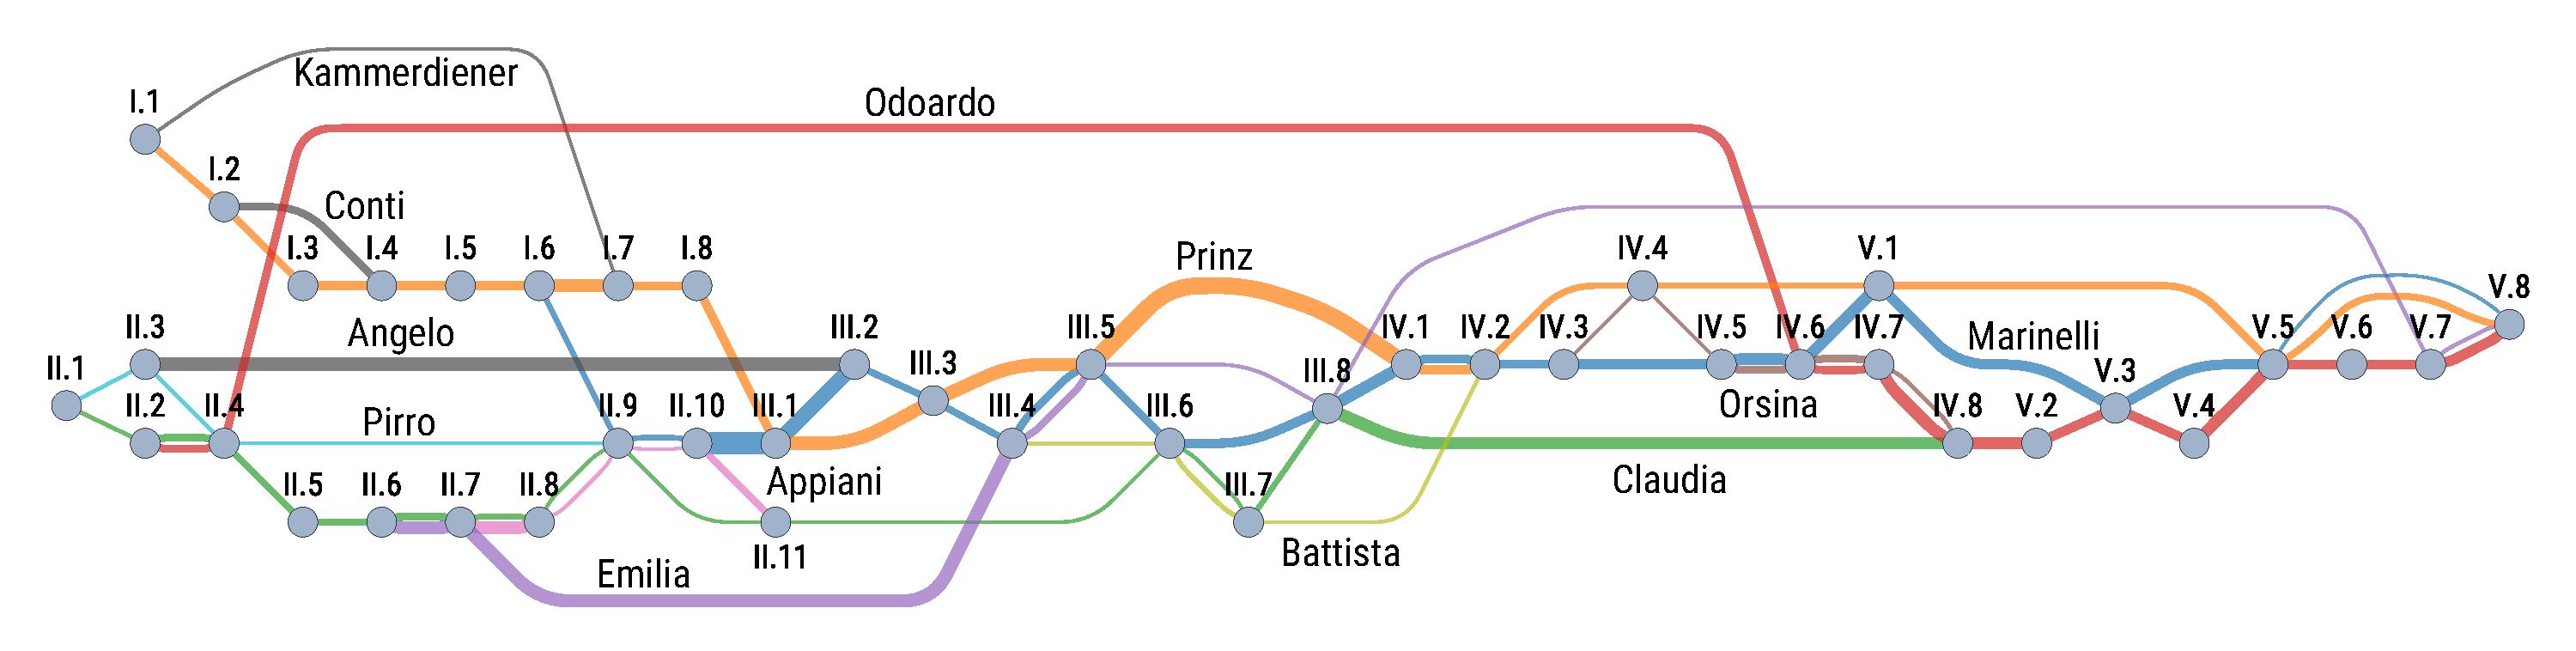
\includegraphics[width=23cm]{graph.pdf}}
    \caption{Einbettung des Situationsgraphen zu \emph{Emilia Galotti}.
        Jede Ecke wird als ein Punkt gezeichnet. Pfeile $r$ werden als Linie von $\alpha(r)$ zu $\omega(r)$ dargestellt, dabei ist der Punkt zu $\alpha(r)$ in der Darstellung immer links vom Punkt zu $\omega(r)$.
    Bis auf Angelo, Conti und den Kammerdiener ist dem Pfad jeder Figur eine eindeutige Farbe zugeordnet. Alle Pfeile der Form $(s_i,s_j, f)$ mit Gewicht $w$ sind dann in der zu $f$ zugehörigen Farbe gezeichnet, und die Dicke des Pfeilzugs ist linear in Abhängigkeit von $w$.}
    \label{fig:situationsgraph}
    \makebox[\textwidth][c]{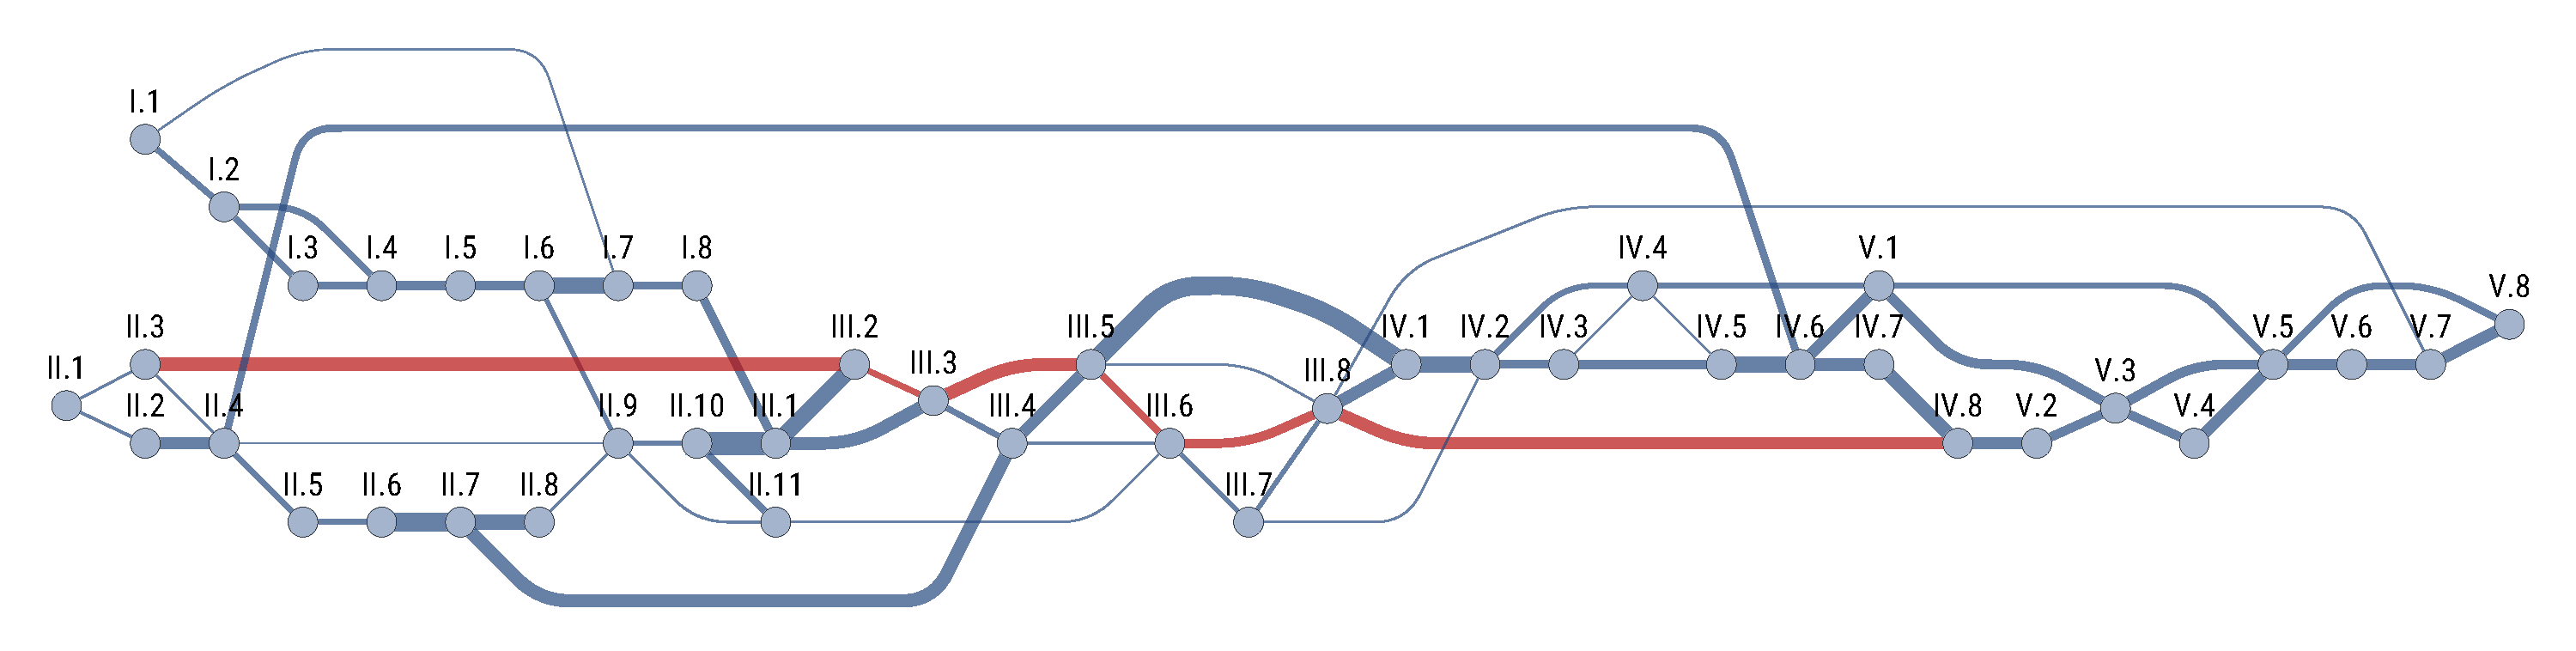
\includegraphics[width=23cm]{graphsim.pdf}}
    \caption{Selbe Einbettung des einfachen Situationsgraphen zu \emph{Emilia Galotti}. Die rot hervorgehobenen Linienzüge entsprechen dem auf S.~\pageref{pos:weg-diskussion} diskutierten Weg.} 
    \label{fig:situationsgraph-einfach}
\end{SidewaysFigure}

Die selbe Abbildung zeigt schon, wie solche Situationsgraphen ein graphischen Überblick über das Werk ermöglichen.
Es sei hier anzumerken, dass sich eine Konfigurationsmatrix in einen ungewichteten Situationsgraph umrechnen lassen kann und umgekehrt – die beiden Darstellungsformen sind im Wesentlichen äquivalent.
Vorteil der Darstellung als Graph liegt dann insbesondere darin, dass Fragen wie \textquote{Wann tritt Odoardo wieder auf, nach seiner Exposition im Akt II.4} leicht beantwortet werden können. % hunspell: acc Odoardo

Auf diese Verwendungsweise als Visualisierung soll aber im Folgenden nicht weiter eingegangen werden.
Stattdessen wollen wir uns näher mit dem eigentlichen Forschungsdesiderat beschäftigen.
Deshalb nehmen wir noch eine Vereinfachung des Situationsgraphen vor, und transformieren diesen in einen \emph{einfachen} gerichteten azyklischen Graph.
Hierzu fassen wir alle parallelen Pfeile in einen einzigen zusammen, und summieren ihre Gewichte.
Abbildung \ref{fig:situationsgraph-einfach} zeigt den einfachen Situationsgraphen für \emph{Emilia Galotti}, hervorgegangen aus entsprechendem Situationsgraphen der Abbildung \ref{fig:situationsgraph}.


\subsection{Kausale Zusammenhänge zwischen Situationen}


Nun können wir uns der ersten Behauptung zuwenden:
Ein Pfeil $r$ von $s_i$ nach $s_j$ im einfachen Situationsgraph zeigt an, dass (mindestens) eine \emph{Handlung} in Situation $s_i$ kausal eine Handlung in Situation $s_j$ verursacht hat, bzw. ein Effekt dieser Handlung ist.
Wie stark dieser Zusammenhang ist, wird durch die Gewichtung des Pfeils deutlich.

Diese Behauptung soll durch folgende Überlegungen plausibilisiert werden. 
Zunächst halten wir folgende einfache Beobachtungen fest, die sich aus der Definition des Graphen ergeben:
\begin{enumerate*}
    \item Die Situation $s_i$ geschieht werks-chronologisch vor Situation $s_j$. % hunspell: acc werks-chronologisch
    \item Die Konfigurationen dieser beiden Situationen überschneiden sich.
        Für diese Figuren ist $s_j$ der unmittelbar folgende Auftritt nach $s_i$.
\end{enumerate*}

Die Beobachtung (i) hängt eng mit dem \textquote{Prinzip der Sukzession} zusammen.
Pfister argumentiert, dass ohne ein \textquote{vermittelndes Kommunikationssystem} ein narratives Nachtragen von Handlungen die Ausnahme bildet, und daher die Präsentationsabfolge der Handlungsabfolge entspricht.\autocite[Vgl.][273]{pfister_drama:_2001}
Damit erlaubt Beobachtung (i) einen restriktiven Charakter.
Die notwendige (zunächst aber nicht hinreichende) Voraussetzung wird gesichert, dass $s_j$ auch tatsächlich \emph{in der Gesamthandlung} nach $s_i$ stattfindet.
Also dass Handlungen in $s_i$ überhaupt einen kausalen Effekt auf die Handlungen in $s_j$ haben kann.

Auch wenn die folgende Argumentation eher unscharf sind, dürfte Beobachtung (ii) wesentlich zur Behauptung beitragen.
Eine Teilmenge an Figuren ist sowohl in $s_i$ als auch $s_j$ präsent.
Damit wird zum Einen eine \emph{Informationsweitergabe} im inneren Kommunikationssystem plausibel.\autocite[Vgl.][Absch.~3]{pfister_drama:_2001}
Informationen werden von dieser Figur in $s_i$ empfangen und ggf., aber szenisch frühestens, in $s_j$ vergeben.
Diese Informationsvergabe sollte einen Effekt auf die Informiertheit der anderen Figuren haben.
Zum anderen haben die in $s_i$ empfangenen Informationen einen Einfluss auf die jeweilige Figur und ihre Handlungen in der darauf folgenden Situation $s_j$. (Wie bspw. bei einem Befehl und dessen Ausführung vorliegt.)
Das Ausmaß dieser beiden Effekte hängt jedenfalls rudimentär mit der Replikenlänge von $f$ in den Situationen zusammen, was durch das Pfeilgewicht reflektiert wird.
In dem hier vorliegenden Fall gilt $w(r) = \sum_{f\in F} \min \{ \rho(s_i, f), \rho(s_j, f) \}$.
Ein kausaler Effekt durch Figur $f$ wird also dann festgemacht, wenn diese in beiden Situationen viel spricht.


\subsection{Handlungssequenzen – Wege im Situationsgraph}\label{sec:wege}


Es liegt unmittelbar nahe, die eben gewonnene Behauptung über Pfeile auf \emph{Wege} im einfachen Situationsgraph $G_\text{sim}$ auszudehnen.
Sei $P=(s_{i_0}, r_1, s_{i_1}, r_2, s_{i_2}, \dots, r_k, s_{i_k})$ ein Weg in $G_\text{sim}$. 
Da der Pfeil $r_1$ von Situation $s_{i_0}$ nach $s_{i_1}$ zeigt, schließen wir aus voriger Behauptung, dass eine Handlung in $s_{i_0}$ eine Handlung in $s_{i_1}$ bewirkt.
Ebenso bewirkt eine Handlung in $s_{i_1}$ eine in $s_{i_2}$, usw., bis zu einer Handlung in Situation $s_{i_k}$.
Wir können also den Weg $P$ als Zeuge einer Handlungssequenz verstehen, dass einzelne Handlungen aus den Situationen $s_{i_1}, \dots, s_{i_k}$ ein zusammenhängendes \textquote{System chronologischer und kausaler Relationen} bilden, wie in Abschnitt \ref{sec:handlung} beschrieben.
Damit haben wir für die zweite am Anfang genannte Behauptung argumentiert.
Hieraus folgt, dass wir plausible Handlungssequenzen im Drama finden können, wenn wir den Situationsgraphen gegeben haben. 

\label{pos:weg-diskussion}Abbildung \ref{fig:situationsgraph-einfach} zeigt den einfachen Situationsgraph von \emph{Emilia Galotti} mit einem hervorgehobenen Weg.
Die Überlegungen scheinen zumindest für diese Instanz zutreffend zu sein.
Der Weg von II.3 zu V.5 erklärt tatsächlich eine zumindest überwiegend plausible Handlungssequenz:
Angelo wird von Pirro über den Weg der Hochzeitsgesellschaft zum Trauungsort informiert (II.3); Mutmaßlich erlaubt ihm diese Information den erfolgreichen Überfall auf die Hochzeitskutsche, und gegenüber Marinelli Erfolg zu verkünden (III.2–3).
Dadurch wird die überlistete Emilia vom Prinzen empfangen und wird in ein Nebenzimmer geführt (III.5).
Entsprechend muss Marinelli die Intrige selbst weiter verfolgen und empfängt Claudia Galotti  (III.6).
Er erklärt ihr, dass der Prinz schon um Emilia beschäftigt ist, aber Claudia erkennt Marinelli als denjenigen, mit welchem Appiani im Streit vor seinem Tod war.
Sie schöpft Verdacht und drängt zu Emilia (III.8).
Nach ihrer Begegnung ist sich Claudia daher sicher, dass Emilia den Prinzen auf Distanz halten würde, und beteuert dies Odoardo (IV.8).



\section{Segmentierung in Handlungssequenzen – Disjunkte Wegüberdeckungen}\label{sec:segmentierung}

Voriger Abschnitt machte Korrespondenz zwischen Handlungssequenzen im Drama, und Wegen im entsprechenden einfachen Situationsgraph $G_\text{sim}$ plausibel.
Diese Einsicht wird nun logisch fortgeführt.
Durch graphentheoretische Methoden kann eine Segmentierung der Gesamthandlung in Handlungssequenzen errechnet werden.
Hierfür werden zunächst im ersten Teil theoretische Überlegungen durchgeführt, welche diese Behauptung stützen.
Im Anschluss wird im zweiten Teil diese endgültige Operationalisierung anhand Goethes Werks \emph{Götz von Berlichingen} vorgeführt.

\subsection{Zur Operationalisierung}

Zerlegen wir $G_\text{sim}$ in disjunkte Wege, erreichen wir nach bisherigen Überlegungen eine Segmentierung des Dramas.
Deshalb seien im Folgenden \emph{gewichtsmaximale disjunkte Wegüberdeckungen} in $G_\text{sim}$ betrachtet.
Wir verwenden dabei folgende Definition:
\emph{Das Gewicht einer disjunkten Wegüberdeckung $\mathcal{P}$ eines mit $w$ gewichteten Graphen ist $w(\mathcal{P}) = \sum_{P\in\mathcal{P}} \sum_{r\in R(P)} w(r)$. Also das gesamte Gewicht aller durchlaufener Pfeile aller Wege in $\mathcal{P}$.}
Unter dieser Definition von Gewicht ist das Bestimmen einer gewichtsmaximalen disjunkten Wegüberdeckung in gewichteten einfachen gerichteten azyklischen Graphen algorithmisch effizient lösbar, indem bspw. auf das Problem des Matchings maximalen Gewichts reduziert wird.\footnote{Dieses Ergebnis ist mathematische Folklore. Siehe auch \cite[761]{cormen_introduction_2009} für den ungewichteten Fall.}
Damit ist auch zu gewichtetem $G_\text{sim}$ eine gewichtsmaximale Wegüberdeckung $\mathcal{P}^*$ effizient berechenbar.

Es folgen nun Hinweise, dass folgende Operationalisierung das in der Einleitung gewünschte Ziel erreicht:
Eine gewichtsmaximale disjunkte Wegüberdeckung $\mathcal{P}^*$ kann eine sinnvolle Segmentierung der Gesamthandlung in Handlungssequenzen liefern.
Hieraus sollte eine Plot-Strukturierung ersichtlich werden.
Vgl. Seite \pageref{page:plot-segmentierung}.
Dazu drei Punkte:

\begin{enumerate*}[itemjoin=\\\hspace*{\parindent}] % hunspell: acc itemjoin
    \item Zunächst folgt aus der Definition von Wegüberdeckungen, dass jeder Ecke (Situation) ein Weg zugeordnet ist.
        Damit sind also auch alle Handlungen dieser Situation in einer Sequenz vertreten.
        Das ist offenbar eine notwendige Bedingung für eine geeignete Segmentierung in Handlungssequenzen.
        Wege $(s_i)$ der Länge 0 sollen hier nicht weiter stören, und als Sequenzen interpretiert werden, welche nur aus den Handlungen von $s_i$ bestehen.
        Auch klar ist, dass verdeckte Handlungen ausgespart bleiben, da diese in Situationen höchstens narrativ vermittelt werden. 

    \item Die Wegüberdeckung ist disjunkt, also sind alle Handlungen einer Situation (Ecke) genau einer und der gleichen Sequenz (Weg) zugeordnet. 
        Diese Einschränkung ist eher problematisch, da dies allgemein in Dramen nicht der Fall ist.
        Als da aber Ecken bzw. Pfeile die kleinste Einheit des Modells darstellen, müssen wir diese Einschränkung treffen.

    \item Unter allen Wegüberdeckungen hat $\mathcal{P}^*$ das größte Gewicht.
        Zum Einen haben daher die Pfeile zwischen Situationen einer Sequenz möglichst hohes Gewicht.
        Nach vorigem Abschnitt sind die Sequenzen daher kausal stark zusammenhängend.
        Zum Anderen wird das Gewicht der Pfeile zwischen den Wegen/Sequenzen von $\mathcal{P}^*$ minimiert.
        Daraus sollte sich ergeben, dass die entstandene Segmentierung tatsächlich \textquote{sinnvoll} im Sinne unserer Zielsetzung ist, vgl. Abschnitt \ref{sec:handlung}:
        Eine möglichst grobe Segmentierung in jeweils stark zusammenhängende Sequenzen.
\end{enumerate*}




\subsection{Evaluation an einer beispielhaften Analysen}

\begin{SidewaysFigure}
    \centering
    \makebox[\textwidth][c]{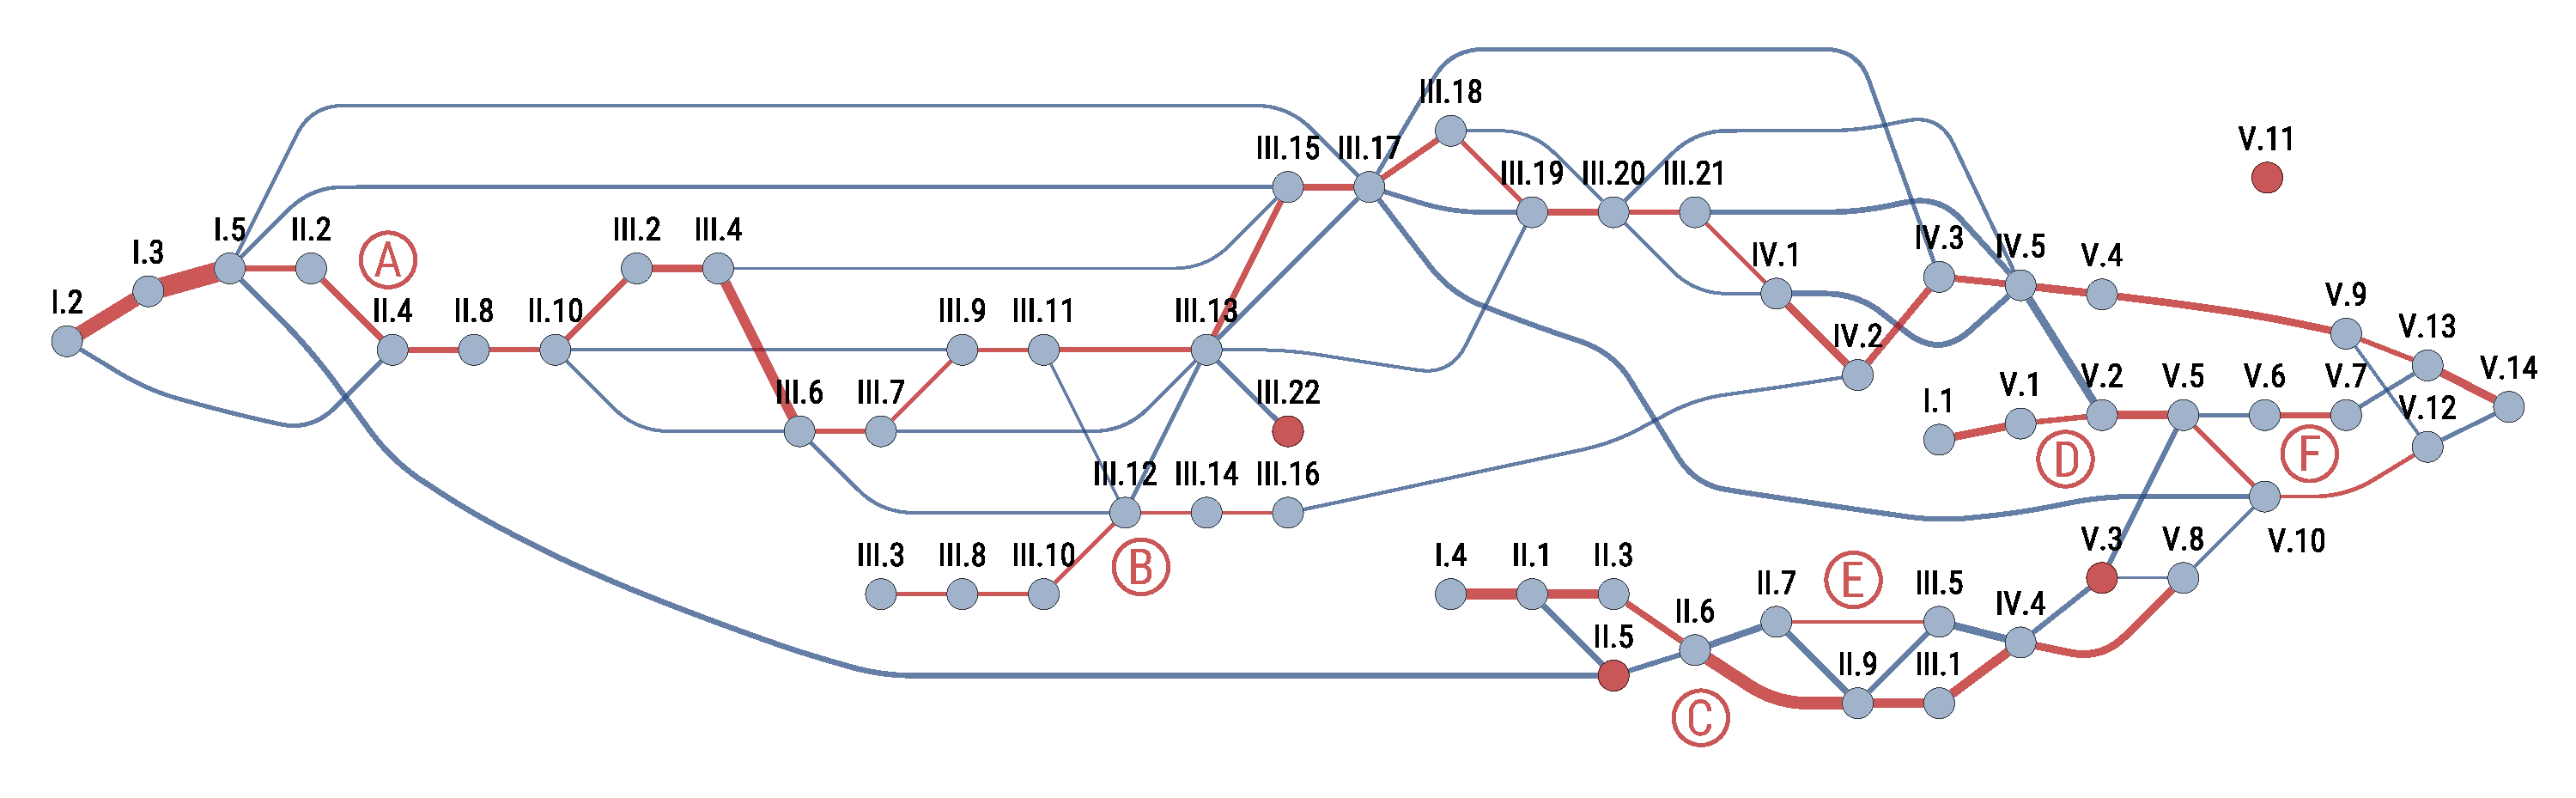
\includegraphics[width=23cm]{graphsim-götz.pdf}}
    \caption{Einbettung des einfachen Situationsgraphen $G_\text{sim}$ zu \emph{Götz von Berlichingen}.
        Wieder sind Ecken als Punkte und Pfeile als Linien visualisiert, Letztere sind von links nach rechts zu lesen.
        Zur besseren Sichtbarkeit ist die Dicke eines Pfeils $r\in R(G_\text{sim})$ proportional zu $w(r)^{2/3}$.
        Ein Pfeil $r$ ist rot hervorgehoben genau dann wenn $r$ von einem Weg $P\in\mathcal{P}^*$ durchlaufen wird.
        Eine Ecke $s$ ist rot hervorgehoben genau dann wenn $s$ von einem Weg $P\in\mathcal{P}^*$ der Länge 0 durchlaufen wird.}
    \label{fig:situationsgraph-götz}
\end{SidewaysFigure}

Die eben durchgeführten Überlegungen wollen wir nun anhand Goethes \emph{Götz von Berlichingen} vorführen und testen.
Die Wahl dieses Werks lässt sich anhand Klotz' Klassifikation als offenes Drama motivieren: 
hier präsentiert sich \textcquote[323]{pfister_drama:_2001}{die Geschichte nicht mehr als geschlossenes, hierarchisches Ganzes}.
Wegen dieser strukturellen Offenheit können wir \emph{Götz} als für die Operationalisierung \emph{schweres Beispiel} verstehen.
Ferner eignet sich die folgende Vorführung auch für einen Vergleich mit Trilckes Netzwerkanalyse des \emph{Götz}.
Er verwendete dabei Figurennetzwerke.\autocite[222--236]{trilcke_social_2013} % hunspell: acc Trilckes

Der für \emph{Götz} zugehörigen Situationsgraph wird aus der TEI-Edition des \emph{GerDraCor} bestimmt, wie im Fall von \emph{Emilia Galotti}.\footnote{
Die TEI-Edition steht dabei vor ähnlichen Schwierigkeiten wie Trilcke:
Erstens treten im \emph{Götz} Kollektive auf, welche in der TEI-Edition wie bei Trilcke als jeweils ein Akteur codiert werden.
Zweitens ist ebenso unklar, ob nicht namentlich genannte Figuren identisch sind oder nicht.
Während Trilcke anhand qualitativ-interpretativer Sichtung des Haupttextes Ambiguitäten aufgelöst hat, scheint die TEI-Edition in jeder neuen Szene eine neuer Akteur angesetzt worden zu sein.
Diese Arbeit übernimmt diese Auszeichnungen.
\cite[Vgl.][Fn.~77]{trilcke_social_2013}.
Drittens, unabhängig von Trilcke, wurden in der TEI-Edition des \emph{GerDraCor} die Szenen V.8 und V.9 fälschlicherweise zusammengelegt, vgl. Zeile 7315. Dies wurde händisch korrigiert. 
}
Durch die in den vorigen Abschnitten beschriebenen Verfahren erreichen wir den einfachen Situationsgraphen $G_\text{sim}$ sowie die dazugehörige gewichtsmaximale disjunkte Wegüberdeckung $\mathcal{P}^*$.
Die Überdeckung besteht aus neun Wegen.
Sechs Wege haben die Länge $>0$, welche wir wie in Abbildung \ref{fig:situationsgraph-götz} nach absteigender Länge mit (A)–(F) benennen.
Drei Wege haben Länge $0$, diese überdecken jeweils Situationen II.5, III.22, V.11.
Die einzelnen Wege können hier aus Platzgründen nicht so ausführlich beschrieben werden wie in Abschnitt \ref{sec:wege} für \emph{Emilia Galotti} durchgeführt wurde.
Stattdessen beschränken wir uns auf einige Beobachtungen zum Situationsgraphen und dieser Segmentierung.

\emph{Zu (A):} Der längste Weg dieser Überdeckung scheint relativ schlüssig eine Handlungssequenz um die Partei Götzens zu erklären, zumindest aber thematisch.
Das ist im ersten Teil die Handlung um Jagsthausen, die Festnahme Götzens, und dessen Rückzug aus Bamberg auf seine Burg.
Fragwürdig ist die Verbindung zum zweiten Teil (ab V.4), in der insbesondere Elisabeth letzte Hilfe für Götz zu erwirken versucht.
Ebenso wird die gesamte Sequenz regelmäßig von Situationen unterbrochen, die nicht im engeren Sinne in einem kausalen Zusammenhang stehen.
Beispielsweise II.11 \textquote{Bauernhochzeit}, oder die Exposition Lerses in III.6.
Ferner ist die eigentliche Situation der Festnahme Götzens (III.22) überhaupt nicht Teil vom Weg (A), denn die Handlung wird dort in einer Mauerschau narrativ vermittelt.

\emph{Zu (B):} Dieser Weg kann zweifelsfrei der Handlung um den Hauptmann der Reichsexekution zugeordnet werden.
Problematisch im Rahmen des Situationsgraphen ist aber, dass die kausalen Wechselwirkungen zwischen dieser Sequenz und jener aus (A) im Graphen nicht angezeigt werden.
Das suggeriert eine nicht vorhandene kausale Isolation der beiden Sequenzen.
Dies ist hier insbesondere dem Umstand geschuldet, dass die Gefechte im dritten Akt zeitlich verdeckt sind, und narrativ nachgetragen werden, vgl. dazu auch Abschnitt \ref{sec:situationen}.

\emph{Zu (C) und (E):} Erster Weg kann als die Sequenz um die Bamberger Partei verstanden werden.
Weislingen wird überlistet, sich gegen Götz zu stellen, und er erwirkt die Reichsacht.
Anschließend wird der kausale Zusammenhang aber diffus, und bezieht sich eher auf Adelheids Plan, Weislingen zu vergiften.
Die eindeutige Konsequenz in V.10 wird dann aber Weg (D) zugeordnet.
Auch die Ausreißer (E), II.5 und V.3 sind schwer zu erklären.
Aber auch genauso schwer ist in diesem thematischen Teil des Dramas eine klare dramaturgische Struktur festzumachen.
Die Einlage der V.11 \textquote{In einem finstern engen Gewölbe} interpretiert das Modell als isoliert. % hunspell: acc finstern
Dass diese Einlage thematische und bis zu kausale Relationen mit dem Rest ausbildet, wird dagegen vom Modell nicht angezeigt.

\emph{Zu (D) und (F)}: Grundsätzlich scheint das Modell nur schwer in der Lage zu sein, ab Akt V nachvollziehbare Handlungssequenzen zu liefern.
Weg (D) bezieht sich bis V.5 auf die Bauernrebellion, springt dann aber zum Tod Weislingens (V.10), anstatt mit Weg (F) fortzufahren.
Dieser bezieht sich auf Götzens Flucht und anschließende Gefangennahme.
Intuitiv viel naheliegender wäre, wenn V.5–V.6 und V.8–V.10 Teil der Überdeckung wären.
Dass stattdessen Pfeil V.5–V.10 Teil der Überdeckung ist, lässt sich vermutlich durch zwei Eigenheiten der Datenlage zu erklären: zum einen ist V.5 \textquote{Bei einem Dorf} eine Szene, welcher eigentlich keiner Situation entspricht, denn Weislingen tritt erst ganz zum Schluss kurz auf.
Zum anderen verzerrt Weislingens lange Replik in dieser Szene die tatsächlich bestehenden kausalen Relationen zu V.6.


\section{Fazit}

Die Arbeit befasste sich mit dem von Trilcke et~al. ausformulierten Forschungsdesiderat, Methoden in der literarische Netzwerkanalyse zu entwickeln, welche eine quantitative Plot-Analyse in Dramen ermöglicht.
Hierzu präsentierte die Arbeit den \emph{Situationsgraph} als ein mathematisches Modell, was die Konfigurationsstruktur eines dramatischen Werks abbildet, ähnlich zu Konfigurationsmatrizen.
Zentraler Unterschied zu bisherigen Ansätzen ist, dass im Situationsgraph nicht Figuren, sondern die Situationen (bzw. Szenen) als Ecken im Graph gewählt werden.
Schon die Visualisierung dieses Situationsgraphen ermöglicht einen Überblick über die syntagmatische Struktur des Dramas.

Im Rahmen dieses Forschungsdesiderats machte die Arbeit zum Ersten plausibel, dass in diesem Situationsgraphen sich kausal verkettete Handlungssequenzen ablesen lassen können.
Zum Zweiten wurde durch oberflächliche literaturtheoretische Überlegungen eine Operationalisierung motiviert, welche einen Vorschlag zur Plot-Strukturierung errechnet.
Hierzu werden algorithmische Methoden auf den Situationsgraphen angewandt.
Ergebnis ist eine Segmentierung in untereinander abgeschlossene Handlungssequenzen.

Diese Operationalisierung wurde anhand Goethes Dramas \emph{Götz von Berlichingen} vorgeführt. Im überwiegenden Maße ließen sich im Ergebnis kausal bzw. thematisch abgetrennte Handlungssequenzen erkennen.
Dennoch wurden  auch Grenzen der Operationalisierung sichtbar.
Nichtsdestotrotz ist dieses eine \textquote*{positive} Ergebnis nicht repräsentativ.
Es ist explizit kein Indiz dafür, dass diese Operationalisierung für alle dramatischen Texte ähnlich gut arbeite.
Eine rigorose Evaluation der hier vorgeschlagenen Operationalisierung setzt einen großen repräsentativen Test-Korpus voraus,
sodass die darin annotierten \textquote*{wahren} Plot-Strukturen mit den Errechneten vergleichen werden können.\autocite[Vgl.][608]{jannidis_computergestuetzte_2017}
Ein solches geeignetes annotiertes Test-Korpus existiert aber gegenwärtig nicht.

Als Ausblick bieten sich also zwei weitere Beschäftigungen mit dem hier vorgeschlagenen Modell an:
Erstens, enger mit der \textquote*{traditionellen} Literaturwissenschaft verknüpft, kann durch eine bewusstere Wahl von Beispielwerken die Mächtigkeit des Modells weiter untersucht werden.
Es können z.\,B. Werke herausgesucht werden, für welche das Modell sehr schlechte Ergebnisse liefert.
Folgt man Moretti, so kann eine Weiterentwicklung bzw. Korrektur des Verfahrens – immer gekoppelt am Plot-Konzept – auch Einsichten zum Begriff Plot liefern.\autocites[Vgl.][13]{moretti_operationalizing:_2013}[Vgl.][]{trilcke_small_2020}

Näher an der Praxis der \eng{Digital Humanities}, lässt sich Zweitens das hier vorliegende Modell vergleichend und unabhängig vom Konzept Plot analysieren: % hunspell: Humanities
Wir folgen hier Überlegungen von Trilcke und Fischer, und verstehen den Situationsgraphen \emph{an sich} als das eigentliche \textquote{epistemische Ding} – nicht das repräsentierte Werk.
Damit fällt die Korrespondenz zu Plot zwar weg, dann aber kann ein Situationsgraph (bzw. deren gewichtsmaximale Wegüberdeckung) als \emph{Element} eines großen Korpus von Situationsgraphen verstanden werden.\autocite[Vgl.][]{trilcke_literaturwissenschaft_2018}
Das digitale Korpus \emph{GerDraCor} induziert beispielsweise einen solchen Korpus von Situationsgraphen, indem die digitalen Editionen in Situationsgraphen umgerechnet werden.
Hierauf können dann mit statistischen Methoden Regularitäten und Ausreißer erkannt werden.
Insbesondere können die einzelnen Graphen mit dem Korpus in Beziehung gesetzt werden.
\textquote{Wie viele Wege hat die gewichtsmaximale Wegüberdeckung eines Situationsgraphen des Korpus \emph{im Durchschnitt}?} wäre beispielsweise eine unmittelbar naheliegende Fragestellung.


\printbibliography\clearpage

\end{document}
